En la literatura se pueden encontrar trabajos que abordan la noción de recuperación de información con diferentes semánticas. Por ejemplo, en \cite{BasuRoy:2010:CEC:1807167.1807258} se propone construir paquetes asociados a un ítem central. Un escenario de aplicación podría ser un usuario comprador de un teléfono celular (ítem central) que dispone de cierto presupuesto al que se le ofrecen paquetes que incluyen otros items relacionados tales como funda, tapa, parlantes, cargador, etc.

En \cite{Xie:2010:BOB:1864708.1864739} se sugiere reemplazar una clásica lista de las mejores $k$ recomendaciones de una búsqueda por los mejores $k$ paquetes recomendados. Por ejemplo, podría aplicarse para un turista que está interesado en sugerencias de lugares o puntos de interés para su viaje, dispone de determinado tiempo y presupuesto y maneja una noción de compatibilidad entre items (a lo sumo 3 museos, recorrido menor a cierta distancia, etc). Si cada atracción tiene asociado un ranking, la idea es ofrecer los mejores $k$ paquetes de atracciones de tal manera que en cada paquete se respete el presupuesto y la compatibilidad entre items.

Ninguno de los trabajos mencionados tiene en cuenta la diversidad entre los paquetes sugeridos, formalizando la recuperación de la información como un problema de {\em clustering} que sólo considera la compatibilidad entre items. Como alternativa, en \cite{compositeRetrival} se propone conjugar en el conjunto de paquetes sugeridos al usuario las nociones de diversidad, similitud y compatibilidad.

A continuación se describen brevemente las características de los algoritmos propuestos en \cite{compositeRetrival}.

\begin{itemize}

\item {\em Produce and Choose} (PAC): Utiliza un esquema de dos fases, donde en la primera se producen paquetes válidos y en la segunda se eligen $k$ entre ellos. Para la producción de paquetes se implementaron dos algoritmos de {\em clustering}, uno basado en {\em clustering} jerárquico aglomerativo (C-HAC) y el segundo en {\em k-means clustering} (BOBO, por Bundles One-By-One). Para la segunda fase se adaptaron heurísticas de la literatura para el problema {\em Maximum Edge Subgraph}.

En C-HAC inicialmente cada ítem forma un {\em cluster} unitario y luego sucesivamente en cada iteración se elige un par de {\em clusters} para ser unidos y generar un {\em cluster} válido, es decir que cumpla las restricciones de complementariedad y no supere el presupuesto $\beta$. El algoritmo finaliza cuando no existe un par de {\em clusters} que pueda ser unido en un {\em cluster} válido o se alcance una condición de parada (por ejemplo número de {\em clusters} generados). Como criterio de elección de los {\em clusters} a unir se busca maximizar la función $Score$, que es la suma de las similitudes de todos los items del par candidato. Este criterio de unión sólo presta atención a la similitud intra-paquete, lo que hace que, cuando se busca una alta diversidad, el conjunto de paquetes generados de esa forma no sea necesariamente bueno.

El método \texttt{BOBO-c}, está inspirado en k-means. En términos simples, consiste en generar $c*k$ {\em clusters} del conjunto de $n$ items. El algoritmo comienza con todos los items del conjunto $I$ como posibles \emph{pivotes} $P$. Se selecciona un pivote de $P$ y con los elementos de $I$ se genera un {\em cluster} válido ``alrededor" de éste. En caso que el {\em cluster} generado sea suficientemente bueno (su valor intra supera un parámetro $\mu$) se agrega al conjunto de paquetes candidatos y los items del {\em cluster} se eliminan de $P$. La generación de {\em clusters} continúa hasta que se cumpla el criterio de parada que es la generación de $c*k$ {\em clusters}. Con BOBO-c pueden quedar items excluidos de los paquetes generados, por lo que se desarrolló una variante del método, llamado BOBO-E' (por Exhaustivo) que logra que todos los items pertenezcan a un paquete. Para esta producción se modificó el criterio de parada hasta que el conjunto de pivotes $P$ sea vacío. Para grandes bases de datos los tiempos de ejecución de esta variante BOBO-E' resulta impracticable.

Al finalizar la producción de paquetes comienza la etapa de selección, en la cual se deben seleccionar los $k$ paquetes que formarán la solución (Selección simple). El problema de seleccionar los paquetes que maximizan la función objetivo se traduce en encontrar en un grafo completo $G$ cuyos vértices representan los paquetes (con pesos asociados dados por sus valores intra) y cuyas aristas tienen como peso los valores inter, el subgrafo de $k$ vértices de mayor peso (considerando los pesos de los vértices y aristas). Para ello se implementó un algoritmo goloso, en el cual se selecciona iterativamente del conjunto de paquetes aquél que maximiza la función objetivo evaluada en los paquetes hasta el momento seleccionados. Notemos que en las primeras iteraciones de esta selección el valor inter-paquetes es despreciable con respecto a la suma de los valores intra-paquete. Esto hace que cuando se quiere privilegiar la diversidad de paquetes en la solución (valores bajos de $\gamma$) ésta no sea una buena estrategia.

Por la forma de generar la solución que tienen las heurísticas tipo {\em Produce and choose} (construir una cantidad suficiente de paquetes y luego seleccionar un subconjunto de éstos), es de esperar que las soluciones generadas se enfoquen más en valorar la parte intra-paquete que la inter-paquetes.

\item {\em Cluster and Pick} (CAP): También sigue un esquema de dos fases. En la primera se busca un $k$-{\em clustering} (un {\em cluster} no es necesariamente un paquete válido) y luego en la segunda se selecciona un paquete válido dentro de cada uno de los {\em clusters} generados en la primera etapa.

\item Método IP: Se presenta un modelo de programación lineal entera que resuelve el problema de forma exacta. Los tiempos de ejecución de este enfoque lo hacen prohibitivo para grandes instancias.

\end{itemize}

Los algoritmos propuestos son evaluados en \cite{compositeRetrival} sobre dos bases de datos reales. Una de ellas se refiere a atracciones turísticas en 10 ciudades europeas, donde por cada una de estas instancias se consideran 20 atracciones. El segundo conjunto de datos se compone de opiniones sobre restaurantes en 149 ciudades proveniente de Yahoo! Local. El número de restaurantes en cada ciudad varía de 300 a 2000.

De la experimentación presentada en \cite{compositeRetrival}, se concluye que las mejores soluciones se obtienen con los algoritmos que primero agrupan los ítems en paquetes válidos y luego seleccionan paquetes dentro de este agrupamiento (PAC). 

A continuación se presentan alternativas a los algoritmos descriptos recientemente, así como también procedimientos de búsqueda tabú que mejoren la calidad de las soluciones obtenidas.

\section{Produce-and-Choose}
El algoritmo para aproximar a la solución \texttt{Produce-and-Choose} genera una cierta cantidad de paquetes y luego seleccionar los que pertenecerán a la solución.

Los parámetros del algoritmo son los del problema: $I$ el conjunto de ítems, $\alpha$ el atributo complementario, $f: 2^{I} \rightarrow \rm I \!R$ la función de presupuesto, $\beta$ el limite del presupuesto, $\gamma$ para ponderar si se quiere paquetes más cohesivos o no y $k$ la cantidad de paquetes a generar. El algoritmo devuelve un conjunto de paquetes válidos.

\begin{algorithm}[H]
\begin{algorithmic}[1]
\REQUIRE {$I,\alpha,f,\beta,k,\gamma$}
\ENSURE Conjunto válido de $k$ paquetes
\STATE $cand \leftarrow ProduceBundle(I,\alpha,f,\beta)$
\STATE $G \leftarrow BuildBundleGraph(cand)$
\RETURN $ChooseBundles(k,\gamma,G)$
\end{algorithmic}
\caption{Produce-and-Choose}\label{alg:PAC}
\end{algorithm}

La función \texttt{ProduceBundle} genera un conjunto de paquetes candidatos, más adelante se analizan distintas estrategias. \texttt{BuildBundleGraph} recibe el conjunto de paquetes candidatos y devuelve un grafo completo con peso en las aristas y en los vértices. Cada vértice representa un paquete del conjunto de candidatos y el peso del vértice es el valor intra, mientras que el peso de las aristas representa el valor inter entre los paquetes que le asocia. Finalmente la función \texttt{ChooseBundles} busca el subgrafo-k que maximice el peso de las vértices y aristas, también se analizan distintas estrategias. Los vértices del subgrafo-k son los paquetes que pertenecen a la solución.\\

La estructura de estos algoritmos permiten introducir mejoras en sus dos fases: generación y selección de paquetes.
\subsection{Generación de paquetes}
La generación de paquetes se puede realizar a través de un proceso de agrupación de un conjunto de objetos que son parecidos. Este proceso conocido como agrupamiento, que consiste en juntar objetos basándose en la información que estos describen o en sus relaciones. El objetivo es que los objetos del grupo sean similares entre sí y diferentes de los objetos de los restantes grupos. Cuanto mayor es la similitud dentro del conjunto (intra) y mayor la diferencia entre ellos (inter) el agrupamiento será mejor.

No existe una definición formal de que es un grupo correctamente constituido porque es muy complejo realizar esta definición. Por ejemplo, para los veinte puntos de la figura \ref{res:img-howToCluster} existen tres (o más) formas de agruparlos que son válidas. Si se permite que los grupos estén acoplados, entonces la estructura más razonable es en la que existen dos grupos. Pero la división de los dos grupos en tres subgrupos es más intuitiva para el ojo humano. Tampoco es irracional decir que los puntos pertenecen a cuatro conjuntos. Entonces la mejor definición depende del tipo de dato y del resultado esperado.

\begin{figure}[H]
  \centering
   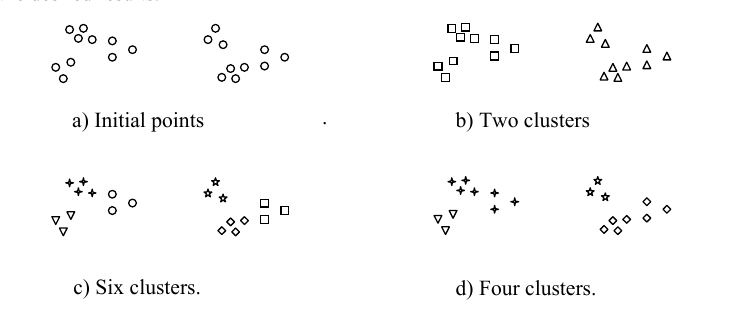
\includegraphics[width=0.8\textwidth]{img/howToCluster.png}
   \caption{}
   \label{res:img-howToCluster}
\end{figure}
En este trabajo el agrupamiento esta definida para que cada grupo contenga la máxima cantidad de items sin exceder el presupuesto. La agrupación se realiza por la similitud de los objetos, que se obtiene a través de la función de similitud, para que los items dentro del grupo sean lo más parecido posible y así obtener paquetes coehsivos.

Existen varios algoritmos de agrupamiento, los cuales se pueden categorizar entre los particionales y los jerárquicos. Los métodos particionales re ubican iterativamente los objetos moviéndolos de un grupo a otro. Generalmente, estos métodos, requieren que la cantidad de grupos a generar sea preestablecido. Los métodos jerárquicos construyen los grupos mediante la partición recursiva de los grupos de objetos y no requieren preestablecer una cantidad pre definica anteriormente.

En este trabajo se implementó un algoritmo de cada categoría. Del método jerárquico se desarrolló el algoritmo \textit{constrained hierarchical agglomerative clustering}, mientras que para el método de partición el algoritmo \textit{Bundles One-By-One}.

\subsubsection{Bundles One-By-One}
El método \texttt{BOBO-k}, que está inspirado en k-means, consiste en generar $k$ paquetes del conjunto de $n$ ítems. El algoritmo comienza con todos los items del conjunto $I$ como posibles pivots $P$. Se selecciona un pivote de $P$ y con los elementos de $I$ se genera un paquete válido alrededor de este, en caso que el paquete generado sea suficientemente bueno se agrega al conjunto de candidatos y los ítems del paquete se eliminan de $I$. La generación de paquetes continúa hasta que se cumpla el criterio de parada, generar de $k$ paquetes válidos. Con \texttt{BOBO-k} pueden quedar ítems excluidos de los paquetes generados, por lo tanto se desarrolló una variante del método que es el \texttt{BOBO-Ex} (Ex de \textit{exhaustive}) en el cual todos los items pertenecen a un paquete. Para esta producción se modificó el criterio de parada hasta que el conjunto de pivotes $P$ sea vacío.\\

\begin{algorithm}[H]
\begin{algorithmic}[1]
\REQUIRE {$I,\alpha,f,\beta,\mu,\text{ cantidad de paquetes }c$}
\ENSURE Conjunto válido de paquetes
\STATE $pivots \leftarrow I$
\STATE $cand \leftarrow \emptyset$
\WHILE {$ \left|C\right| < c\ and\ P \neq \emptyset$}
	\STATE $pivot \leftarrow SelectPivot(pivots)$
	\STATE $bundle \leftarrow BuildBundle(pivot,I,\alpha,f,\beta)$
	\IF {$Score(bundle) \geq \mu$}
		\STATE $cand \leftarrow cand \cup \left\{bundle\right\}$
		\STATE $I \leftarrow I \setminus \left\{bundle\right\}$
		\STATE $pivots \leftarrow pivots \setminus \left\{pivot\right\}$
	\ELSE
		\STATE $pivots \leftarrow pivots \setminus \left\{pivot\right\}$
	\ENDIF
\ENDWHILE
\RETURN $cand$
\end{algorithmic}
\caption{BOBO-k}\label{alg:bobo}
\end{algorithm}

La función \texttt{selPivote} selecciona el pivote del conjunto de pivotes, en este trabajo se siguió con la recomendación de \cite{newSimilarity} que la selección sea aleatoria. La función \texttt{BuildBundle} genera un paquete a partir del pivote. Se trata de una función que implementa un algoritmo goloso dado que que en cada iteración se agrega al paquete que se genera el ítem del conjunto $I$ que maximiza la función intra $f$ y que cumple con las restricciones de la complementaridad y el presupuesto. La función \texttt{Score} calcula el valor intra del paquete. Se dice que un paquete es suficientemente bueno si el valor intra supera el umbral establecido por $\mu$.

\subsubsection{Constrained hierarchical agglomerative clustering}
El agrupamiento jerárquica se clasifica entre los algoritmos \textit{aglomerativo} y \textit{divisivo}. En el aglomerativo inicialmente cada objeto pertenece a un grupo unitario y luego sucesivamente se unen un par de grupos hasta que todos se hayan unido en un único gran grupo que contenga a todos los objetos, este algoritmo es conocido como \textit{hierarchical agglomerative clustering} (HAC). El divisorio comienza con un único grupo al que todos los objetos pertenecen y recursivamente se realiza una división del grupo hasta obtener grupos unitarios.

Comúnmente HAC es visualizado como un dendrograma, como se ve en la figura ~\ref{des:Dendrogram}, cada unión se representa por una línea horizontal y la coordenada Y es la similitud en la que los dos grupos han sido unidos. Por ejemplo la unión del grupo que contiene a \textit{Indiana tobacco lawsuit} con el perteneciente a \textit{Suits against tobacco firms}, es con la similitud aproximada de 0,7. Luego el grupo resultante se une con el que contiene a \textit{Lawsuit against tobacco companies} con la similitud 0,47. Sucesivamente se realizan la unión de estos grupos hasta que quede uno solo.

Ascendiendo desde la capa inferior hasta obtener un único grupo el dendrograma permite reconstruir la historia de las uniones de los grupos. Un supuesto fundamental en el algoritmo HAC es que es monótono, lo que significa que si la unión sucesiva de grupos con las similitudes es $s_1,s_2,\ldots,s_n$ entonces se tiene que $s_1 \geq s_2 \geq \ldots \geq s_n$.

\begin{figure}[H]
  \centering
    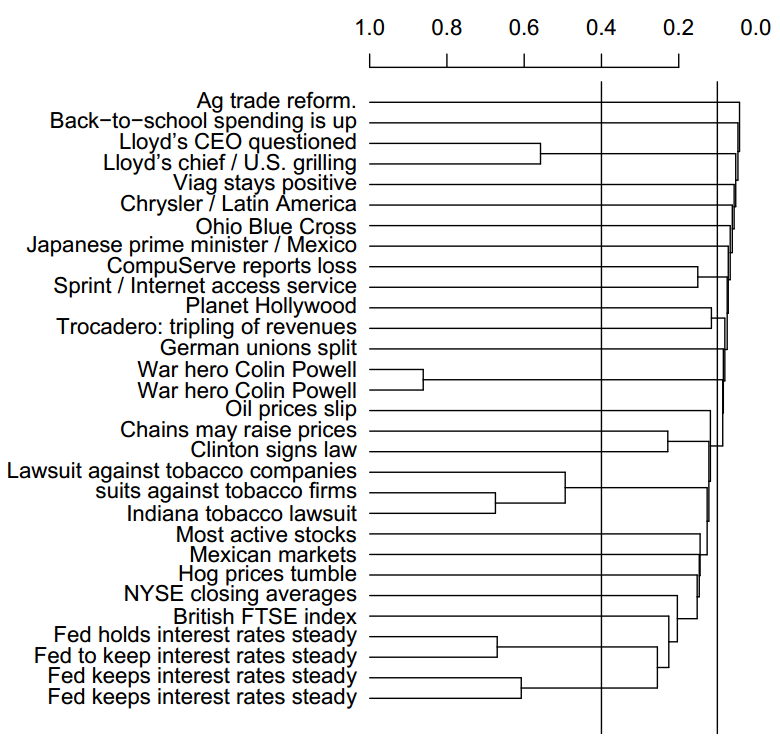
\includegraphics[width=1\textwidth]{img/Dendrogram.png}
  \caption{dendrograma}
  \label{des:Dendrogram}
\end{figure}

\textit{Constrained hierarchical agglomerative clustering} (C-HAC) es una modificación que se realiza sobre HAC para que nunca se realice la unión de los grupos $S_1$ y $S_2$ si el grupo resultante $S_1 \cup S_2$ es inválido, o sea sí el grupo resultante no cumple con las restricciones de similitud o el costo del paquete supera el presupuesto. El algoritmo C-HAC que se presenta a continuación, en este trabajo se denomina \texttt{Simple C-HAC}, es el que se propone en \cite{compositeRetrival}.

\begin{algorithm}[H]
\begin{algorithmic}[1]
\REQUIRE {$I,\alpha,f,\beta,\gamma,\text{ cantidad de paquetes }c$}
\ENSURE Conjunto válido de paquetes
\STATE $cand \leftarrow \bigcup_{i \in I}\left\{i\right\}$
\WHILE {$ \left|cand\right| > c$}
	\STATE $bestScore \leftarrow -\infty$
	\STATE $bestCandidate \leftarrow \emptyset$
	\FOR{$\text{each}\ S_i\in cand$}
		\FOR{$\text{each}\ S_j\in cand; S_i \neq S_j$}
			\IF {$ValidMerge(S_i,S_j,\alpha,f,\beta)$} \label{validMerge}
				\IF {$Score(S_i \cup S_j) \geq bestcore$} \label{score}
					\STATE $bestScore \leftarrow score(S_i \cup  S_j)$
					\STATE $bestCandidate \leftarrow \left\{S_i,S_j\right\}$
				\ENDIF
			\ENDIF
		\ENDFOR
	\ENDFOR
	\IF {$bestCandidate = \emptyset$}
		\BREAK
	\ENDIF
	\STATE {$cand \leftarrow cand \setminus \left\{S\right\}$ $(\forall S \in bestCandidate)$}
	\STATE $cand \leftarrow cand \cup bestCandidate $
\ENDWHILE
\RETURN $cand$
\end{algorithmic}
\caption{Simple C-HAC}\label{alg:SimpleC-HAC}
\end{algorithm}

El algoritmo ejecuta $N - c$ pasos donde se unen los dos grupos más similares que forman un grupo válido. En cada paso se realiza una comparación entre todos los grupos. Por lo tanto el orden de complejidad de \texttt{Simple C-HAC} es $\mathcal{O}(N^{3})$. En cuanto a la función \textit{Score} que se utiliza para decidir qué {\em clusters} unir sólo considera el valor intra-paquete, por lo que es considerado un criterio de unión local.\\

Para salvar estas debilidades aquí se propone la siguiente alternativa inspirada en una propuesta de \cite{MRS}.\\

Con el fin de incluir información inter-paquete en la selección del par de {\em clusters} a unir, se define la función Intra-Inter en reemplazo de la función $Score$ como se indica a continuación. Dados dos {\em clusters} $C_i$ y $C_j$ sean

$$A(C_i,C_j) = \sum_{u \in C_i, v \in C_j}{s(u,v)},$$

$$E(C_i,C_j)=\max_{u \in C_i, v \in C_j}{s(u,v)} \qquad \mbox{ y}$$

$$\mbox{Intra-Inter}(C_i,C_j) = \gamma A(C_i,C_j) + t (1-\gamma) E(C_i,C_j)$$

De esta manera el {\em cluster} resultante incrementará el valor intra y se habrán unido dos {\em clusters} con alta similitud favoreciendo la dispersión en el {\em clustering} final. El factor $t$ intenta equilibrar los dos términos de esta sumatoria, ya que de lo contrario el segundo resultará siempre despreciable con respecto al primero. En este trabajo el valor que se le asigna a $t$ corresponde a la cantidad de similitudes que se suman en A, o sea $\frac{(\#C_i + \#C_j) \cdot (\#C_i + \#C_j - 1)}{2}$  

Un punto clave es el costo computacional del cálculo de la función Intra-Inter. Para evitar realizar el cálculo desde cero de $A$ y $E$ para todo par de {\em clusters} en todas las iteraciones de la etapa \emph{Produce} del algoritmo, se  mantienen estructuras con esos valores, cuya actualización se realiza en tiempo constante a partir de las siguientes relaciones entre la iteración $r$ y la $r-1$:

$$A^r(C_i \cup C_j, C_s) = A^{r-1}(C_i,C_s) + A^{r-1}(C_j,C_s) \quad \mbox{ y}$$

$$E^r(C_i \cup C_j,C_s) = \max (E^{r-1}(C_i,C_s),E^{r-1}(C_j,C_s))$$

El valor de la función Intra-Inter para cada {\em cluster} es almacenado en orden decreciente en una cola de prioridad. La implementación de colas de prioridad permite el borrado e inserción en $O(\log n)$, resultando la complejidad total del algoritmo $O(n^2 log n)$.\\

Por el orden de complejidad del algoritmo \texttt{Simple C-HAC}  en escenarios donde la agrupación se tenga que hacer entre miles de objetos el tiempo de ejecución será tan elevado que el algoritmo es improductivo. Para contemplar estos escenarios se implemento el algoritmo \texttt{Efficient C-HAC} que la complejidad es $\mathcal{O}(N^{2}\lg n)$. La similitud entre los grupos se guarda en colas de prioridad en orden decreciente, entonces la cola $P\left[k\right].max()$ devuelve el grupo de mayor similitud con el k-ésimo grupo. Luego de combinar los grupos $\omega_{k_{1}}$ y $\omega_{k_{2}}$, $\omega_{k_{1}}$ se utiliza como la representación. Para $\omega_{k_{1}}$ se calcula la similitud con el resto de los grupos y se actualiza en las colas de similitud. Para identificar entre dos grupos que la unión es invalida por alguna de las restricciones, en las colas de similitud el valor de la similitud es $-1$.

\begin{algorithm}[H]
\begin{algorithmic}[1]
\REQUIRE {$I,\alpha,f,\beta,\gamma$}
\ENSURE Conjunto válido de paquetes
\FOR{$\text{each}\ S_i\in I$}
	\FOR{$\text{each}\ S_j\in I$}
		\IF {$validMerge(S_i,S_j,\alpha,f,\beta)$} 
			\STATE $C[i][j].sim \leftarrow Score(S_i \cup S_j)$
		\ELSE
			\STATE $C[i][j].sim \leftarrow -1$
		\ENDIF
		\STATE $C[i][j].index \leftarrow j$
	\ENDFOR
	\STATE $I[i] \leftarrow 1$
	\STATE {$P[i] \leftarrow $ priority queue for $C[i]$ sorted on sim}
	\STATE {P[i].Delete(C[i][i]) (se elimina así mismo de la pila)}
\ENDFOR
\STATE $A \leftarrow []$
\FOR {$k \leftarrow 1$ to $I.length$}
	\STATE $k_1 \leftarrow \max_{k:I[k]=1}{P[k].max().sim}$
	\IF {$validMerge(S_i,S_j,\alpha,f,\beta)$}
		\BREAK
	\ENDIF
	\STATE $k_2 \leftarrow P[k_1].max().index$
	\STATE $A.Append(\left\langle k_1,k_2 \right\rangle)$
	\STATE $I[k_2] \leftarrow 0$
	\STATE $P[k_1] \leftarrow []$
	\FOR {$i$ with $I[i]-1 \vee i \neq k_1$}
		\STATE $P[i].Delete(C[i][K_1])$
		\STATE $P[i].Delete(C[i][k_2])$
		\IF {$validMerge(S_i,S_j,\alpha,f,\beta)$}
			\STATE $C[i][k_1].sim \leftarrow Inter-Intra(i,k_1 \cup k_2,\gamma)$
			\STATE $C[k_1][i].sim \leftarrow Inter-Intra(i,k_1 \cup k_2,\gamma)$
		\ELSE
			\STATE $C[i][k_1].sim \leftarrow -1$
			\STATE $C[k_1][i].sim \leftarrow -1$
		\ENDIF
		\STATE $C[i][k_1].index \leftarrow i$
		\STATE $C[k_1][i].index \leftarrow i$		
		\STATE $P[i].Insert(C[i][k_1])$
		\STATE $P[K_1].Insert(C[k_1][i])$		
	\ENDFOR
\ENDFOR

\RETURN $A$
\end{algorithmic}
\caption{Efficient C-HAC}\label{alg:Efficient C-HAC}
\end{algorithm}

\subsection{Selección de paquetes}
Al finalizar la producción de paquetes comienza la etapa de selección de los mismos, en la cual se deben seleccionar los $k$ mejores paquetes para la solución. El problema de seleccionar los que maximizan la función objetivo se traduce en encontrar en el grafo completo G con peso en los nodos y vértices (el peso de los nodos representa la calidad de los paquetes y el peso de las aristas es la distancia entre los nodos) el k-subgrafo de mayor peso (considerando los nodos y vértices).

Formalmente el problema de encontrar el subgrafo de máximo peso de nodos y vértices con k nodos, consiste en dado el grafo $ G = (V,E) $, la funciones de peso $\psi : E \rightarrow \Re$ y $\omega : V \rightarrow \Re$, el entero $ k \leq |V| $ y el real $\gamma \in [0,1]$. La salida es el conjunto $V' \subseteq V$ tal que $|V'| = k$ que maximiza el peso de los nodos y vértices del subgrafo $G' = (V', E')$ ponderado por el parámetro $\gamma$.

\begin{equation}
\gamma \sum_{v \in V'}{\omega(v)} + (1 - \gamma) \sum_{(u,v) \in E'}{\psi(u,v)}
\end{equation}

El problema de encontrar el máximo k-subgrafo con pesos en los nodos y vértices, se puede reducir al problema ya conocido de hallar el k-subgrafo más denso\cite{SubgraphProblem}. Transformando en la instancia del problema original la función del peso de los vértices por:
 
\begin{equation}
\omega(u,v) = \dfrac{\gamma}{2( k - 1)} (\omega(u) + \omega(v)) + (1 - \gamma)\psi(u,v) 
\end{equation}

A esta nueva instancia del problema se le aplica la heurística golosa, del artículo \cite{compositeRetrival}, en la que en cada iteración se remueve el nodo con menos peso en las aristas.

\begin{algorithm}[H]
\begin{algorithmic}[1]
\REQUIRE $k,\gamma,\text{ el grafo con peso en los vértices y aristas }G=(V,E) \text{ donde }\forall S \in V / \omega(S) = \sum_{u,v \in S}{s(u,v)}$ y $\forall (S_i,S_j) \in E / \psi(S_i,S_j) = 1 - \max_{u \in S_i, v \in s_j}{s(u,v)}$
\ENSURE Conjunto de k bundles
\STATE $\omega(u,v) = \dfrac{\gamma}{2( k - 1)} (\omega(u) + \omega(v)) + (1 - \gamma)\psi(u,v)$
\STATE $S \leftarrow V$
\WHILE {$ \left|S\right| > k$}
\STATE $u \leftarrow \min_{u \in S}{\sum_{v \in S}{\omega(u,v)}}$
\STATE $S \leftarrow S \setminus  \left\{u\right\} $
\ENDWHILE
\RETURN $C$
\end{algorithmic}
\caption{Selección de paquetes}\label{alg:chooseBundles}
\end{algorithm}

En este trabajo se propone otra heurística para la selección que consiste en ir seleccionando iterativamente los paquetes de la solución. En cada iteración se elije al paquete que maximiza la función objetivo, a diferencia del algoritmo ~\ref{alg:chooseBundles}, multiplicada por un coeficiente para ponderar la parte inter de la función. Esta ponderación se realiza porque el peso del nodo (parte intra de la función) es mayor al peso de la arista (parte inter). Con este equilibrio se asegura que en las primeras iteraciones el valor del inter no sea despreciable en comparación con el valor del intra al momento de realizar la selección.

Sea $B$ el conjunto de paquetes producidos y $S \subseteq B$ el conjunto de paquetes seleccionados en la iteración $i$ se agrega a la solución el paquete que cumple con:

\begin{equation}
\max_{b \in (B/S)}{\dfrac{k}{|S|}} \gamma \sum_{v \in \left\{b\right\} \cup S}{\omega(v)} + \dfrac{k * (k-1)}{|S| * (|S|-1)} (1-\gamma) \sum_{v,w \in \left\{b\right\} \cup S}{\psi(v,w)}
\end{equation}

\begin{algorithm}[H]
\begin{algorithmic}[1]
\REQUIRE $k,\gamma, \text{el grafo con peso en los vértices y aristas } G=(V,E) \text{ donde } \forall S \in V / \omega(S) = \sum_{u,v \in S}{s(u,v)} y \forall (S_i,S_j) \in E / \psi(S_i,S_j) = 1 - \max_{u \in S_i, v \in s_j}{s(u,v)}$
\ENSURE Conjunto de k bundles
\STATE $S \leftarrow V$
\WHILE {$ \left|S\right| < k$}
\STATE $c \leftarrow \max_{b \in (B/S)}{\dfrac{k}{|S|}} \gamma \sum_{v \in \left\{b\right\} \cup S}{\omega(v)} + \dfrac{k * (k-1)}{|S| * (|S|-1)} (1-\gamma) \sum_{v,w \in \left\{b\right\} \cup S}{\psi(v,w)}$
\STATE $S \leftarrow S \cup \left\{c\right\}$
\STATE $B \leftarrow B \setminus \left\{c\right\}$
\ENDWHILE
\RETURN $S$
\end{algorithmic}
\caption{Selección de paquetes proporcional}\label{alg:algSelProp}
\end{algorithm}

\section{Algoritmo goloso}
Un algoritmos goloso es un tipo de heurística que construye la solución iterativamente seleccionando en cada paso la opción óptima local, esperando así lograr una solución óptima al finalizar la ejecución. No siempre encuentra la solución óptima pero son muy usados por su sencillez y velocidad de la ejecución.

Por la forma de generar la solución que tiene la heurística \texttt{Produce-and-choose} de construir una cantidad suficiente paquetes y luego seleccionar un conjunto se puede suponer que las soluciones se enfocan más en la parte intra que inter, esto motivo a realizar a implementar una heurística.

El algoritmo goloso que se propone comienza con con los $k$ paquetes de la solución vacíos e iterativamente se agrega un item, que no pertenece a la solución, en el paquete que maximiza la función objetivo y sin violar las restricciones del problema. El algoritmo finaliza cuando por alguna restricción no es posible agregar más objetos a la solución. Un posible escenario de este algoritmo es que a la solución $S$ se le agrega el ítem $i$ obteniedo así la solución válida $S'$ y que el valor de la función objetivo de $S$ sea mayor que el de $S'$, ya que se la prioridad es que la solución resultante tenga la mayor cantidad de ítems posibles.

\begin{algorithm}[H]
\begin{algorithmic}[1]
\REQUIRE {$I,\alpha,f,\beta,k,\gamma$}
\ENSURE Conjunto válido de paquetes
\STATE $\omega(S) = \sum_{b \in S}{\sum_{u,v \in b}{\gamma s(u,v)}} + \sum_{b_1,b_2 \in S}{(1-\gamma) (1-\max_{u \in b_1, v \in b_2}{s(u,v)})}$
\STATE $cand \leftarrow \bigcup_{1 \ldots k}\emptyset$
\STATE $isComplete \leftarrow False$
\WHILE {$isComplete = False$}
  \STATE $bestScore \leftarrow -\infty$
  \STATE $bestCandidate \leftarrow \varnothing$
  \STATE $bestBundle \leftarrow \varnothing$
  \FOR {$\text{each}\ elem \in I$}
    \FOR {$\text{each}\ bundle \in cand$}
      \IF {$validMerge(bundle,\{elem\},\alpha,f,\beta)$}
        \STATE $score \leftarrow \omega((Cand \setminus \left\{bundle\right\}) \cup \left\{bundle \cup \left\{elem\right\}\right\})$
        \IF {$score > bestScore$}
          \STATE $bestScore \leftarrow score$
          \STATE $bestBundle \leftarrow bundle$
          \STATE $bestCandidate \leftarrow elem$
        \ENDIF
      \ENDIF
    \ENDFOR
  \ENDFOR
	\IF {$bestCandidate \neq \varnothing$}
		\STATE $cand \leftarrow (cand \setminus \left\{bestBundle\right\}) \cup \left\{bundle \cup \left\{bestCandidate\right\}\right\}$
		\STATE $I \leftarrow I \setminus \left\{bestCandidate\right\}$
	\ELSE
		\STATE $isComplete \leftarrow True$
	\ENDIF
\ENDWHILE
\RETURN $cand$
\end{algorithmic}
\caption{Algoritmo heurística golosa}\label{alg:algHeuGol}
\end{algorithm}

\section{Búsquedas Tabú}
Las búsquedas locales consisten en moverse de solución en solución, aplicando cambios a la solución candidata hasta encontrar una mejor solución o satisfacer un criterio de parada. Los algoritmos comienzan a partir de una solución válida y en cada iteración se mueve a una solución vecina, esto es posible solo si se pude definir una relación de vecindad en el espacio de soluciones. Como una solución puede tener muchas soluciones vecinas se elige siempre la que maximice (o minimice, según el problema elegido) el criterio seleccionado, esto produce que el algoritmo pueda estancarse en un máximo (ó mínimo) local y nunca pueda salir de él.

\textbf{Tabú search} es una metaheurística para resolver problemas de optimización, de la familia de las búsquedas locales, diseñada para escapar de óptimos locales. Para explorar regiones del espacio de búsqueda que serían dejadas de lado por el procedimiento de búsqueda local, la búsqueda tabú modifica la estructura de vecinos para cada solución a medida que la búsqueda progresa y permite moverse a una solución vecina de menor calidad. De esta manera se permite al algoritmo escapar de máximos (o mínimos) locales.

Las implementaciones de búsqueda tabú utilizan estructuras de memoria, conocidas como listas tabú, que determinan cuáles son las soluciones vecinas permitidas de una solución. Para evitar que soluciones de buena calidad no sean visitadas porque la lista tabú lo prohíbe, se introduce el concepto de criterios de aspiración que permite, bajo ciertas circunstancias, visitar una solución que se encuentra en la lista tabú.

Una de las ventajas que tienen este tipo de metaheurísticas es que no son muy costosas en tiempo de ejecución siempre que la cantidad máxima de iteraciones no sea excesiva, con lo cual se puede ejecutar sin problemas y sin importar de que algoritmo de generación y selección provenga la solución orginal con el fin de intentar mejorarla.

Se implementaron las búsquedas tabú Inter-Paquete e Intra-Paquete. La primera busca encontrar una mejor solución entre la actual y los paquetes ya generados; la otra consiste en mejorar los paquetes con los ítems que quedaron fuera de la solución.

\subsection{Inter-Paquete}
La búsqueda se concibió especialmente para la fase de selección del algoritmo \texttt{Produce and Choose}, es decir en la fase que se selecciona un subconjunto de paquetes de los generados en la fase anterior de producción. De la solución obtenida en la fase de selección se va a realizar la búsqueda tabú con los paquetes generados en la fase de producción con el objetivo de visitar soluciones vecinas y esperando obtener una mejor selección.

Para esta implementación se define que las soluciones vecinas de la solución $S$, son aquellas soluciones que que no contienen el paquete con menor valor Inter de $S$ e incluye un paquete que no pertenece a $S$. El paquete que se saca de $S$ se agrega a la lista tabú durante $n$ iteraciones. Esta lista contiene los paquetes que no pueden ser parte de la solución a visitar. Además se define para el criterio de aspiración, admitir una solución vecina que contiene un paquete que esta en la lista tabú si mejora la función objetivo con respecto a la mejor solución encontrada hasta el momento. 

Los movimientos de la solución $S$ a la solución $S'$ consiste de los siguientes  pasos:
\begin{enumerate}
	\item Quitar de la solución el paquete con menor Inter.
	\item Determinar el paquete centroide de la solución.
	\item Calcular la función objetivo agregando uno de los $K$ paquetes generados más lejos del centroide.
	\item Quedarse con la solución con mayor función objetivo. 
\end{enumerate}

Sea $S$ el conjunto de paquetes de la solucion y B el conjunto de todos los paquetes producidos. El paquete (1) es el más acoplado al de la solución $b_r = \min_{b_1 \in S}{\sum_{b_2 \in S}{\psi(b_1,b_2)}}$. El centroide de (2) es el paquete que tiene mayor similitud entre los restantes de la solución, sin tener en cuenta al indicado a reemplazar, entonces el centroide es:
$$b_c = \min_{b_1 \in S \setminus \left\{b_r\right\}}{\sum_{b_2 \in S \setminus \left\{b_r\right\}}{\psi(b_1,b_2)}}$$
El paquete de (3) se obtiene de $b_n = \min_{b_1 \in S \setminus \left\{b_r\right\}}{\psi(b_1,b_c)}$. Por lo tanto la nueva solución es $S' = (S \setminus \left\{b_r\right\}) \cup \left\{b_n\right\}$. Mientras que el paquete $b_r$ se marca para que no sea seleccionado para las próximas soluciones generadas.
\begin{algorithm}[H]
\begin{algorithmic}[1]
\REQUIRE {$S\text{ solucion},cand\text{ conjunto válido de paquetes},\gamma, MAX\_SOL\text{ cantidad de soluciones vecinas visitadas},MAX\_BUND\text{ cantidad bundles para probar}, ITER\_TABU\text{ iteraciones en tabú}$}
\ENSURE Conjunto válido de paquetes
\STATE $\omega(S) = \sum_{b \in S}{\sum_{u,v \in b}{\gamma s(u,v)}} + \sum_{b_1,b_2 \in S}{(1-\gamma) (1-\max_{u \in b_1, v \in b_2}{s(u,v)})}$
\STATE $UpdateTabu(S) = \left\{ \left\langle b, n-1 \right\rangle  / \left\langle b, n \right\rangle \in S \wedge n-1 > 0 \right\}$
\STATE $Inter(b_1, S) = \sum_{b_2 \in S, b_1\neq b_2}{(1-\max_{u \in b_1, v \in b_2}{s(u,v)})}$
\STATE $Inter(S) = \sum_{b_1, b_2 \in S}{(1-\max_{u \in b_1, v \in b_2}{s(u,v)})}$
\STATE $iteration \leftarrow 0$
\STATE $tabuBundles \leftarrow \emptyset$
\STATE $bestSolution \leftarrow S$
\STATE $visitSolution \leftarrow S$ 
\WHILE {$iteration < MAX\_ITER$}
  \STATE $worstBundle \leftarrow \min_{b \in visitSolution \setminus tabuBundles}{Inter(b, visitSolution)}$
	\STATE $centroidBundle \leftarrow getCentroid(visitSolution)$
	\STATE $bestBundles \leftarrow \text{fetch first MAX\_BUND} \max_{b \in cand \setminus tabuBundles}{Dist(b, centroidBundle)}$
	\STATE $visitSolution \leftarrow \emptyset$
	\FOR {$\text{each}\ aBundle \in bestBundles$}
    \STATE $iterationSolution \leftarrow (visitSolution \setminus \left\{worstBundle\right\}) \cup \left\{aBundle\right\}$
    \IF {$inter(iterationSolution) > inter(nextVisit)$}
			\STATE $visitSolution \leftarrow iterationSolution$
    \ENDIF
  \ENDFOR
	
  \IF {$\omega(visitSolution) > \omega(bestSolution)$}
    \STATE $bestSolution \leftarrow visitSolution$
  \ENDIF
  \STATE $tabuBundles \leftarrow tabuBundles \cup \left\{
	\left\langle worstBundle, ITER\_TABU \right\rangle\right\}$
	\STATE $tabuBundles \leftarrow UpdateTabu(tabuBundles)$
	\STATE $iteration \leftarrow iteration + 1$
\ENDWHILE
\RETURN $bestSolution$
\end{algorithmic}
\caption{Búsqueda tabú sobre paquetes}\label{alg:algBusTabuBundle}
\end{algorithm}

\subsection{Intra-Paquete}
El objetivo de la búsqueda Intra-Paquete es explorar soluciones con paquetes más cohesivos para si hallar una solución con mejor función objetivo. En esta búsqueda los vecinos de la solución $S$ son las soluciones a las cuales se le modifica el paquete de $S$ con menor Intra. La modificación del paquete puede consistir en: agregar un elemento, quitar un elemento o intercambiar un elemento del paquete con otro elemento que no pertenece a la solución, siempre y cuando el nuevo paquete generado sea válido. En esta implementación existen tres listas tabú: una lista de elementos, una de movimientos y una de paquetes. Los elementos que se encuentran en la lista tabú, no pueden ser seleccionados para incluirse en una solución. Los paquetes de la lista, son los que no pueden ser seleccionados para modificar su estructura para una nueva solución y la lista de movimientos contiene los elementos que se intercambiaron de la solución $S$ a  $S'$ para que esos elementos no se vuelvan a intercambiar.

Para evitar ciclar entre las soluciones, por ejemplo si las soluciones visitadas son $S, S_1, \ldots, S_n, S$ para que la próxima no sea $S_1$ es que se agregó la lista tabú de movimientos.

De la solución actual se realiza el movimiento a una nueva solución con los pasos:
\begin{enumerate}
	\item Obtener el paquete, $p$, menos cohesivos de la solución $S$.
	\item Crear el paquete $p'$ válido agregando un elemento que no pertenezca a la solución a $p$.
	\item Crear el paquete $p''$ válido quitando de $p$ el elemento más alejado del centroide.
	\item Crear el paquete $p'''$ válido quitando de $p$ el elemento más alejado del centroide y agregando el elemento que no pertenece a la solución $S$
	\item La solución $S' = \max{S\setminus\{p\}\cup\{p'\}, S\setminus\{p\}\cup\{p''\}, S\setminus\{p\}\cup\{p'''\}}$.
\end{enumerate}

Sea $S$ el conjunto de paquete de la solución e $I$ el conjunto de ítems, el paquete de (1) es $b = \min_{b_1 \in S}{\sum_{v,w \in b_1}{s(v,w)}}$. De $b$ se define el centroide $c$ del paso (2) con $c = \max_{v \in b}{\sum_{w \in b}{s(v,w)}}$. El item de (3) se obtiene de $i = \min_{v \in b}{s(v,c)}$. El item para reemplazar a $i$ es $j = \max_{v \in I \setminus items(S)}{s(v,c)}$. Por lo que la nueva solución se define $S' = (S \setminus \left\{b\right\}) \cup \left\{(b \setminus \left\{i\right\})\cup\left\{j\right\}\right\}$

\begin{algorithm}[H]
\begin{algorithmic}[1]
\REQUIRE {$S\text{ solucion},cand\text{ conjunto válido de paquetes},I,\alpha,f,\beta,k,\gamma, MAX\_SOL\text{ cantidad de soluciones vecinas visitadas},MAX\_BUND\text{ cantidad bundles para probar}, ITER\_TABU\text{ iteraciones en tabú}$}
\ENSURE Conjunto válido de paquetes
\STATE $\omega(S) = \sum_{b \in S}{\sum_{u,v \in b}{\gamma s(u,v)}} + \sum_{b_1,b_2 \in S}{(1-\gamma) (1-\max_{u \in b_1, v \in b_2}{s(u,v)})}$
\STATE $Inter(b_1, S) = \sum_{b_2 \in S, b_1\neq b_2}{(1-\max_{u \in b_1, v \in b_2}{s(u,v)})}$
\STATE $Intra(b) = \sum_{u,v \in b}{\gamma s(u,v)}$
\STATE $UpdateTabu(S) = \left\{ \left\langle b, n-1 \right\rangle  / \left\langle b, n \right\rangle \in S \wedge n-1 > 0 \right\}$
\STATE $iteration \leftarrow 0$
\STATE $tabuBundles \leftarrow \emptyset$
\STATE $tabuElements \leftarrow \emptyset$
\STATE $bestSolution \leftarrow S$
\WHILE {$iteration < MAX\_ITER$}
  \STATE $worstBunlde \leftarrow \min_{b \in visitSolution \setminus tabuBundles}{Intra(b)}$
  \STATE $centroid \leftarrow GetCentroid(worstBunlde)$
  \STATE $faraway \leftarrow GetFarawayElement(worstBunlde,centroid)$
  \STATE $bestElements \leftarrow \text{fetch first MAX\_BUND} \max_{b \in I \setminus tabuElements}{Dist(b, centroidBundle)}$
	\STATE $visitSolution \leftarrow \emptyset$
  \FOR {$anElement \in bestElements$}
		\STATE $newBundle \leftarrow (worstBunlde \setminus \left\{faraway\right\})\cup\left\{near\right\}$
		\STATE $iterationSolution \leftarrow (visitSolution \setminus \left\{worstBunlde\right\}) \cup \left\{newBundle\right\}$
		\IF {$\omega(iterationSolution) > \omega(visitSolution)$}
			\STATE $visitSolution \leftarrow iterationSolution$
		\ENDIF
  \ENDFOR
  \IF {$\omega(visitSolution) > \omega(bestSolution)$}
		\STATE $bestSolution \leftarrow visitSolution$
  \ENDIF
	\STATE $tabuBundles \leftarrow tabuBundles \cup \left\{
	\left\langle worstBunlde, ITER\_TABU \right\rangle\right\}$
  \STATE $tabuElements \leftarrow tabuElements \cup \left\{
	\left\langle faraway, ITER\_TABU \right\rangle\right\}$
	\STATE $tabuBundles \leftarrow UpdateTabu(tabuBundles)$
  \STATE $tabuElements \leftarrow UpdateTabu(tabuElements)$
	\STATE $iteration \leftarrow iteration + 1$
\ENDWHILE
\RETURN $bestSolution$
\end{algorithmic}
\caption{Búsqueda tabú sobre elementos}\label{alg:algBusTabuIntra}
\end{algorithm}
